\documentclass{article}
\usepackage[utf8]{inputenc}

% Incluimos los comandos para ajustar el documento
\usepackage{preamble}

\title{Dimensionado de un lanzador}
\author{Raúl Ordás Collado \\ Alejandro Paz Rodríguez  \\ Guillermo Peña Martínez}
\date{Diciembre 2022}

\begin{document}

% Encabezado
\pagestyle{fancy}
\fancyhf{}
\fancyhead[R]{Vehículos Lanzadores y Misiles \\ Grado en Ingeniería Aeroespacial}

\maketitle

Una vez elegido el número de etapas con las que se diseñará un cohete, debe determinarse el tamaño de cada una de dichas etapas. En base a ello se pide responder a las siguientes cuestiones:

\begin{enumerate}
    \item Dimensione un vehículo lanzador de etapa única capaz de imprimir a una carga de pago de \qty{2000}{kg} una velocidad de \qty{7.8}{km/s}. Considere un impulso específico y una fracción estructural media de las indicadas en la tabla siguiente.
    \item Para la misma carga de pago y velocidad final, dimensione un lanzador de tres etapas bajo la hipótesis de \textit{restricted staging}.
    \item Para la misma carga de pago y velocidad final, determine la masa óptima de cada una de las tres etapas del vehículo lanzador. Se sabe que cada etapa puede construirse con las siguientes características:
        \begin{table}[h]
        \centering
        \begin{tabular}{ccc}
        \hline
                & $I_s$ (s) & $\varepsilon$ \\ \hline
        Etapa 1 & 315     & 0.10     \\
        Etapa 2 & 330     & 0.15     \\
        Etapa 3 & 345     & 0.20     \\ \hline
        \end{tabular}
        \end{table}   
    \item Responder a la siguiente cuestión. A la hora de elegir entre diversas opciones de motorización para cada una de las etapas del vehículo lanzador, ¿qué resulta más conveniente, colocar los sistemas de mayor impulso específico en la primera etapa o en la última?
\end{enumerate}

\section{Solución}
% Primera parte
\subsection{Primera parte}

% Segunda parte
\subsection{Segunda parte}
De la hipótesis de \textit{restricted staging} se obtiene que
 $$ \lambda_{1}=\lambda_{2}=\lambda_{3} $$
Siendo
\[ \lambda_{1}=\frac{m_{02}}{m_{01}-m_{02}} \qquad \lambda_{2}=\frac{m_{03}}{m_{02}-m_{03}} \qquad \lambda_{3}=\frac{m_{PL}}{m_{03}-m_{PL}} \]
Aplicando dichas igualdades se obtiene que
\begin{align*}
    m_{02} & = \sqrt{m_{0}m_{03}}  \\
    m_{03} & =\sqrt{m_{02}m_{PL}} \\
    m_{03} & = \frac{m_{0}m_{PL}}{m_{02}}  
\end{align*}
Gracias a estas expresiones podemos obtener  $m_{02}$ y $m_{03}$ en función de $m_{PL}$ y $\pi_{PL}$
\begin{equation}\label{eq:mass}
    m_{02}=\frac{m_{PL}}{\pi_{PL}^{2/3}} \qquad
    m_{03}=\frac{m_{PL}}{\pi_{PL}^{1/3}}
\end{equation}
Ahora podemos poner $\lambda_{3}$ en función de $\pi_{PL}$
\begin{equation}
    \lambda_{3}=\frac{m_{PL}}{\frac{m_{PL}}{\pi_{PL}^{1/3}}-m_{PL}}=\frac{\pi_{PL}^{1/3}}{1-\pi_{PL}^{1/3}}
\end{equation}
Y sabiendo que $n$ es
$$ n=\frac{1+\lambda}{\varepsilon+\lambda} $$
$$ n_{3}=\frac{1+\frac{\pi_{PL}^{1/3}}{1-\pi_{PL}^{1/3}}}{\varepsilon+\frac{\pi_{PL}^{1/3}}{1-\pi_{PL}^{1/3}}}
=\frac{(1-\pi_{PL}^{1/3})+\pi_{PL}^{1/3}}{\pi_{PL}^{1/3}\varepsilon+\pi_{PL}^{1/3}}
=\frac{1}{\varepsilon-\varepsilon\pi_{PL}^{1/3}+\pi_{PL}^{1/3}}$$
\begin{equation}\label{eq:n3}
    n_{3}=\frac{1}{\varepsilon+\pi_{PL}^{1/3}(1-\varepsilon)}
\end{equation}
De la expresión de la velocidad en el apagado podemos calcular $n_{3}$
\begin{equation}
    v_{bo}=I_{sp}g_{0}\ln{n_{3}^3}
\end{equation}
\begin{equation}
    n_{3}=\exp{\frac{v_{bo}}{3I_{sp}g_{0}}} = \num{2.2325}
\end{equation}
Se puede despejar $\pi_{PL}$ de la expresión \ref{eq:n3}
\begin{equation}
    \pi_{PL}=\left(\frac{\frac{1}{n_{3}}-\varepsilon}{1-\varepsilon}\right)^3 = \num{0.04306}
\end{equation}
Ya podemos obtener el valor de las masas de cada etapa sin más que aplicar \ref{eq:mass} y teniendo en cuenta que $m_{0}=m_{01}$
\[m_{0}=\frac{m_{PL}}{{\pi_{PL}}}=\qty{46449.76}{kg}  \qquad
m_{02}=\frac{m_{PL}}{{\pi_{PL}}^{2/3}}=\qty{16280.42}{kg} \qquad
m_{03}=\frac{m_{PL}}{{\pi_{PL}}^{1/3}}=\qty{5706.21}{kg}\]
\newpage
Al asumir la hipótesis de \textit{restricted staging} se tiene que $\varepsilon=\varepsilon_{1}=\varepsilon_{2}=\varepsilon_{3}$ luego podemos obtener el valor de las masas estructurales de cada etapa como:
\begin{align*}
    m_{E_1} &= \varepsilon(m_{0}-m_{02})= \qty{4525.40}{kg} \\
    m_{E_2} &= \varepsilon(m_{02}-m_{03}) = \qty{1586.13}{kg}  \\
    m_{E_3} &= \varepsilon(m_{03}-m_{PL}) = \qty{555.93}{kg} 
\end{align*}
Para el cálculo de las masas podemos hacerlo intuitivamente mediante la figura \ref{fig:1} que aparece en \cite{curtis}:
\begin{align*}
    m_{p_1} &= m_{0}-m_{E_1}-m_{02} = \qty{25643.94}{kg} \\
    m_{p_2} &= m_{02}-m_{E_2}-m_{03} = \qty{8988.09}{kg}  \\
    m_{p_3} &= m_{03}-m_{E_3}-m_{PL} = \qty{3150.28}{kg}
\end{align*}

\begin{figure}
    \centering
    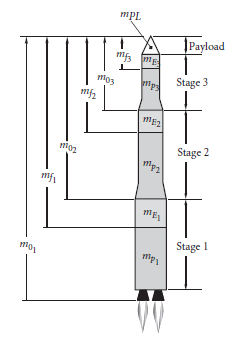
\includegraphics[width=5cm]{imagenes/3etapas.png}
    \caption{Masas en un lanzador de tres etapas}
    \label{fig:1}
\end{figure}
       

% Tercera parte
\subsection{Tercera parte}

Sabiendo que nuestro vehículo lanzador tiene que tener tres etapas, para calcular la masa óptima de cada una de ellas recurrimos al procedimiento descrito en \cite{curtis}, que utiliza el multiplicador de Lagrange, $\eta$, para hacer una optimización restringida en $N$ variables arbitrarias.

Partimos de la definición de masa de la etapa como la suma de la masa estructural y del propelente que lleva individualmente cada una.
\begin{equation} \label{eq:mi}
    m_i = m_{E_i} + m_{p_i}
\end{equation}
Otra expresión a tener en cuenta es la masa estructural como el factor estructural multiplicado por la masa de la etapa.
\begin{equation} \label{eq:mei}
    m_{E_i} = \varepsilon_i (m_{E_i} + m_{p_i}) = \varepsilon_i m_i
\end{equation}

La masa total del vehículo $m_0$ es la suma de las masas de cada etapa y la de la carga útil, $m_{PL}$ que ya conocemos
\begin{equation} \label{eq:m0}
    m_0 = m_{PL} +  \sum_{i=i}^N m_i
\end{equation}
donde $N$ es igual a 3.

Queremos minimizar $m_0$ que es una función que depende en nuestro caso de tres parámetros $m_1$, $m_2$ y $m_3$ a lo largo de otra función que viene dada por
\begin{equation} \label{eq:vbo}
    v_{bo} = I_{sp}g_0 \ln n = \sum_{i=1}^N c_i \ln n_i
\end{equation}

Podemos calcular las velocidades de escape efectivas para cada etapa $c_i$ porque conocemos sus impulsos específicos
\[ c_1 = \qty{3.0902}{km/s} \qquad c_2 = \qty{3,2373}{km/s} \qquad c_3 = \qty{3.3846}{km/s} \]
Las fracciones de masa $n_i$ se calculan en función de las masas de cada etapa como
\begin{equation}
    n_i = \frac{m_{PL} + \sum_{j=i}^{N-i+1} m_j}{\varepsilon_i m_i + m_{PL} + \sum_{j=i}^{N-i} m_j}
\end{equation}
A partir de $n_i$ se despejan las masas por etapa,
\begin{equation} \label{eq:m}
    m_i = \frac{n_i - 1}{1 - n_i\varepsilon_i} \left(m_{PL} + \sum^{N-i}_{j=i+1} m_j \right)
\end{equation}
% Revisar esto
Se realizan manipulaciones algebraicas hasta que la función $\nicefrac{m_0}{m_{PL}}$ queda
\begin{equation}
    \frac{m_0}{m_{PL}} = \prod_{i=1}^N \frac{(1-\varepsilon_i)n_i}{1-\varepsilon_i n_i}
\end{equation}
Se toman logaritmos a ambos lados de la ecuación y se desarrollan hasta quedar en forma de sumas y restas.
\begin{equation}
    \ln\frac{m_0}{m_{PL}} = \sum_{i=1}^N \ln \frac{(1-\varepsilon_i) n_i}{1 - \varepsilon_i n_i} = \sum_{i=1}^N \;[\ln(1-\varepsilon_i) + \ln n_i - \ln(1 - \varepsilon_i n_i)]
\end{equation}

Creamos una nueva función $h$ que incluye el multiplicador de Lagrange y que tiene la forma $h = f + \eta g$ donde $f$ es una función multivariable y $g$ es una curva.
\begin{equation}
    h = \sum_{i=1}^N \;[\ln(1 - \varepsilon_i) + \ln n_i - \ln (1 - \varepsilon_i n_i)] + \eta \left( v_{bo} - \sum_{i=1}^N c_i \ln n_i \right)
\end{equation}
La función $h$ será estacionaria cuando $\partial h/\partial n_i = \partial h/\partial \eta = 0$.
\begin{equation}
\begin{split}
    \frac{\partial h}{\partial n_i} &= \frac{1}{n_i} + \frac{\varepsilon_i}{1 - \varepsilon_i n_i} - \eta \frac{c_i}{n_i} = 0 \\
    \frac{\partial h}{\partial \eta} &= v_{bo} - \sum_{i = 1}^N c_i \ln n_i = 0
\end{split}
\end{equation}
Por un lado vemos que un requisito es que se cumpla la ecuación \ref{eq:vbo} que incluye los factores de carga $n_i$ que podemos despejar a partir de la ecuación anterior.
\begin{equation} \label{eq:n}
    n_i = \frac{c_i \eta - 1}{c_i \varepsilon_i \eta}
\end{equation}
Podemos generalizar la ecuación \ref{eq:vbo} con los factores de carga para despejar $\eta$.  
\begin{equation}
    \sum_{i=1}^N c_i \ln \frac{c_i \eta}{c_i \varepsilon_i \eta} = v_{bo}
\end{equation}

Puesto que es una función no lineal, continua y monótonamente creciente utilizamos el método de Newton incluido en la librería \verb|scipy| para hallar su raíz. Como valor inicial hemos escogido aproximadamente $\nicefrac{1}{\min{c_i}}$ que sabemos que tendrá un valor negativo en la función y por tanto el valor de la raíz de su derivada será siempre positivo para evitar que haya valores negativos en los logaritmos y por tanto que no encuentre una solución.
\[ \eta = \num{0.45855} \]
Con este valor calculamos las fracciones óptimas de masa para cada etapa mediante la ecuación \ref{eq:n}.
\[ n_1 = \num{2.943} \qquad n_2 = \num{2.176} \qquad n_3 = \num{1.778} \]
Podemos calcular las masas de cada etapa con la ecuación \ref{eq:m}.
\[ m_1 = \qty{33369.66}{kg} \qquad m_2 = \qty{7706.27}{kg} \qquad m_3 = \qty{2415.49}{kg} \]
A partir de las ecuaciones \ref{eq:mei} y \ref{eq:mi} podemos hallar las masas en vacío y del propelente, respectivamente.
\[ m_{E_1} = \qty{3336.97}{kg} \qquad m_{E_2} = \qty{1155.94}{kg} \qquad m_{E_3} = \qty{483.10}{kg} \]
\[ m_{p_1} = \qty{30032.70}{kg} \qquad m_{p_2} = \qty{6550.33}{kg} \qquad m_{p_3} = \qty{1932.39}{kg} \]
Las fracciones de carga en cada etapa  son iguales a
\begin{equation*}
    \lambda_i = \frac{m_{PL} + \sum_{j=i+1}^{N-i} m_j}{m_i}
\end{equation*}
\[ \lambda_1 = \num{0.363} \qquad \lambda_2 = \num{0.573} \qquad \lambda_3 = \num{0.828} \]
La masa total del vehículo se calcula con la fórmula \ref{eq:m0}.
\begin{equation*}
    m_0 = \qty{45491.43}{kg}
\end{equation*}
La fracción de carga útil de todo el vehículo es
\begin{equation*}
    \pi_{PL} = \frac{m_{PL}}{m_0} = \num{0.044}
\end{equation*}

Por último, para comprobar que todas las fracciones de masa $n_i$ son mínimos, hacemos las segundas derivadas de $h$ respecto a $n_i$ y comprobamos que, efectivamente, todas son mayores que cero.
\begin{equation}
    \frac{\partial^2 h}{\partial n_i^2} = \frac{\eta c_i (1 - \varepsilon_i n_i) + 2\varepsilon_i n_i - 1}{n_i^2 (1-\varepsilon_i n_i)^2} > 0
\end{equation}

% Cuarta parte
\subsection{Cuarta parte}

\printbibliography[title={Referencias}]

\end{document}


